\documentclass{AnantDocumentation}
\usepackage{tikz}
\usetikzlibrary{shapes.geometric, arrows.meta, positioning, fit, backgrounds}

\backgroundsetup{
	contents=""
}

\title{Audio Watermarking using DWT-DTMT-MLNCML:\\Implementation and Analysis}
\author{Meghadri Ghosh - 2023A3PS0314P \\ Pramit Pal - 2023AAPS0765P \\ Pranav Chandra N. V. - 2023AAPS0013P}

\begin{document}
\maketitle

\section{Approach}

We combined three transforms: MLNCML encrypts the watermark $W \in \{0,1\}^{32 \times 32}$ using coupled logistic maps to produce $W' = W \oplus H_b$ where $H_b$ is generated with $\epsilon=0.3, \mu=3.99$. The audio is segmented into $L_{\text{seg}} = \lceil (N \cdot M) / L_1 \rceil = 256$ blocks. Each segment undergoes 3-level Haar DWT:
\begin{equation}
\text{DWT}^3(\text{segment}) \rightarrow (A_3, D_3, D_2, D_1)
\end{equation}
where $A_3$ contains low-frequency approximation coefficients. We divide $A_3$ into $L_1=4$ sub-blocks and apply DTMT with $K = \min(64, L_2/2)$ Tchebichef polynomial orders:
\begin{equation}
M = T \cdot \text{pa3}, \quad T \in \mathbb{R}^{K \times L_2}
\end{equation}
Moments split into even/odd indices: $M_1 = M[0::2], M_2 = M[1::2]$. We embed bit $b$ by modifying norms:
\begin{equation}
(\sigma_1', \sigma_2') = \begin{cases}
(\bar{\sigma} + \delta, \bar{\sigma} - \delta) & b = 1 \\
(\bar{\sigma} - \delta, \bar{\sigma} + \delta) & b = 0
\end{cases}, \quad \bar{\sigma} = \frac{\|M_1\| + \|M_2\|}{2}, \quad \delta=0.05
\end{equation}
Reconstruction uses inverse DTMT ($\text{pa3}' = T^T M'$) and inverse DWT. Extraction compares $\|M_1\|$ vs $\|M_2\|$ to recover bits, then decrypts: $\hat{W} = \hat{W}' \oplus H_b$. See Figure \ref{fig:flowchart}.

\section{Results}

Table \ref{tab:results} shows robustness against four attacks: LPF (4 kHz) should succeed since we embed in low frequencies, HPF (300 Hz) attacks our weak point, cropping (20\%) tests localized damage, and Gaussian noise (20 dB) tests statistical perturbations.

\begin{table}[h]
\centering
\caption{Attack robustness metrics: SNR (audio quality), BER (bit errors), NC (pattern correlation)}
\label{tab:results}
\begin{tabular}{@{}lccc@{}}
\toprule
\textbf{Attack} & \textbf{SNR (dB)} & \textbf{BER} & \textbf{NC} \\
\midrule
LPF 4000 Hz     & --- & --- & --- \\
HPF 300 Hz      & --- & --- & --- \\
CROP 20\%       & --- & --- & --- \\
Gaussian 20 dB  & --- & --- & --- \\
\bottomrule
\end{tabular}
\end{table}

\section{Key Learnings}

\textbf{Frequency band selection.} Embedding in detail bands ($D_1, D_2, D_3$) created tinny audio—high frequencies are perceptually obvious. Low-frequency $A_3$ works better but remains vulnerable to HPF.

\textbf{Reconstruction isn't perfect.} Haar DWT padding and DTMT truncation ($K = \min(64, L_2/2)$) introduce errors. Hard segmentation creates discontinuities like cutting audio without cross-fading.

\textbf{Metrics vs perception.} 40 dB SNR seems imperceptible but ears detect frequency distortions. Psychoacoustic masking is essential for true imperceptibility.

\textbf{Numerical precision matters.} MLNCML's $2^{100}$ keyspace provides security, but floating-point rounding breaks decryption. Chaotic systems demand exact parameters.

\textbf{Moments provide robustness.} Norm ratios survive attacks because perturbations affect $M_1$ and $M_2$ similarly. Direct coefficient modification fails.

\textbf{Parameter tuning.} $\delta=0.05$ balances robustness and artifacts through trial and error. Future work needs adaptive embedding, error correction, windowing, and better wavelets.

\newpage

\section*{Appendix: System Architecture}

Figure \ref{fig:flowchart} shows how the three transforms work together. The watermark flows through encryption, gets split across audio segments, and embeds into frequency-domain moments. Extraction reverses the process.

\begin{figure}[h]
\centering
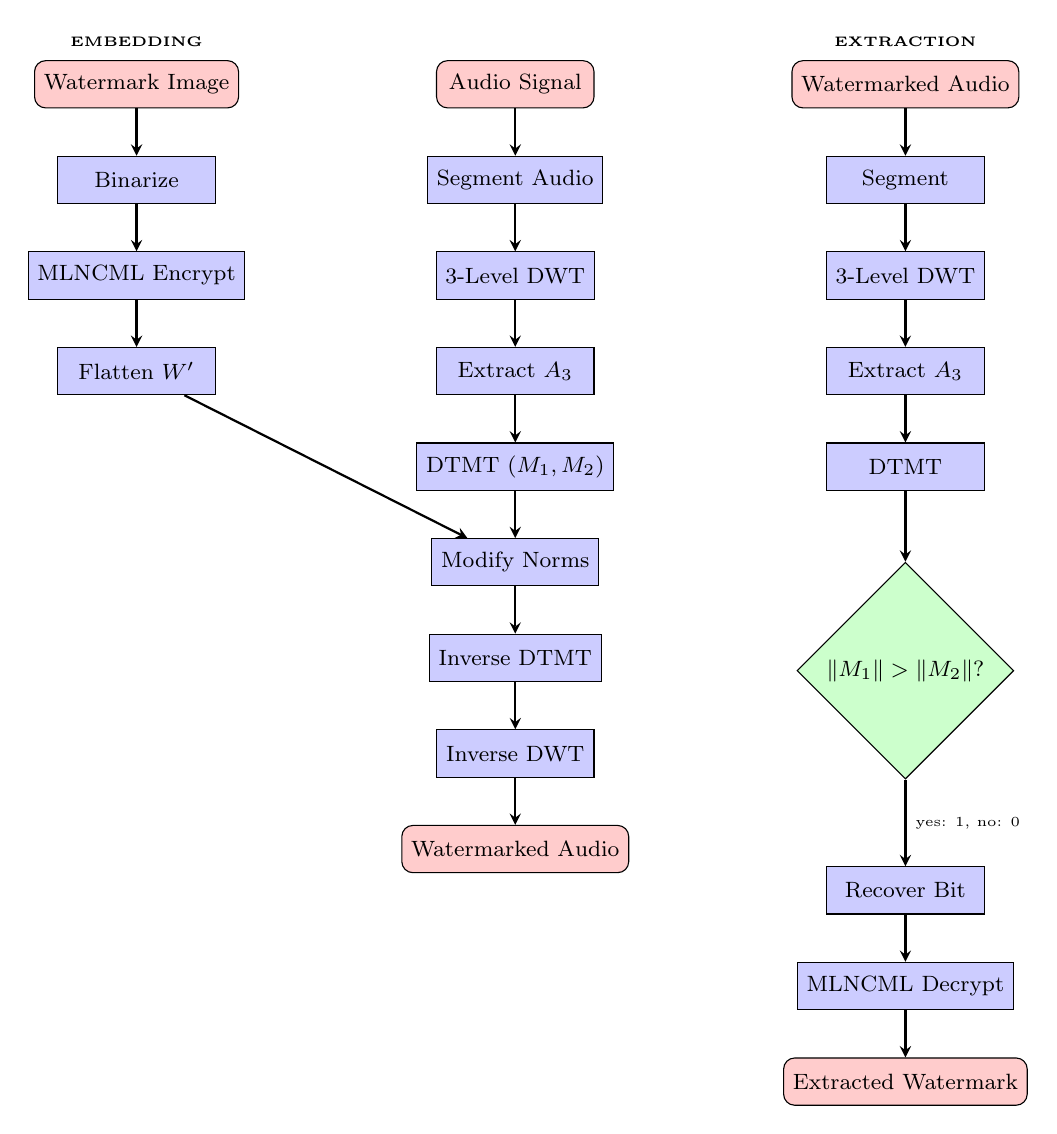
\begin{tikzpicture}[scale=1, every node/.style={transform shape},
    node distance=0.6cm and 1cm,
    startstop/.style={rectangle, rounded corners, minimum width=2cm, minimum height=0.6cm, text centered, draw=black, fill=red!20, font=\footnotesize},
    process/.style={rectangle, minimum width=2cm, minimum height=0.6cm, text centered, draw=black, fill=blue!20, font=\footnotesize},
    decision/.style={diamond, minimum width=1.5cm, minimum height=0.6cm, text centered, draw=black, fill=green!20, font=\footnotesize},
    arrow/.style={thick,->,>=stealth}
    ]
    
    % Embedding path
    \node (img) [startstop] {Watermark Image};
    \node (binarize) [process, below=of img] {Binarize};
    \node (mlncml) [process, below=of binarize] {MLNCML Encrypt};
    \node (flatten) [process, below=of mlncml] {Flatten $W'$};
    
    \node (audio) [startstop, right=2.5cm of img] {Audio Signal};
    \node (segment) [process, below=of audio] {Segment Audio};
    \node (dwt) [process, below=of segment] {3-Level DWT};
    \node (extract) [process, below=of dwt] {Extract $A_3$};
    \node (dtmt) [process, below=of extract] {DTMT ($M_1, M_2$)};
    \node (modify) [process, below=of dtmt] {Modify Norms};
    \node (idtmt) [process, below=of modify] {Inverse DTMT};
    \node (idwt) [process, below=of idtmt] {Inverse DWT};
    \node (watermarked) [startstop, below=of idwt] {Watermarked Audio};
    
    % Extraction path
    \node (wm_audio) [startstop, right=2.5cm of audio] {Watermarked Audio};
    \node (seg2) [process, below=of wm_audio] {Segment};
    \node (dwt2) [process, below=of seg2] {3-Level DWT};
    \node (a3_2) [process, below=of dwt2] {Extract $A_3$};
    \node (dtmt2) [process, below=of a3_2] {DTMT};
    \node (compare) [decision, below=of dtmt2, yshift=-0.3cm] {$\|M_1\| > \|M_2\|$?};
    \node (bit) [process, below=of compare, yshift=-0.5cm] {Recover Bit};
    \node (decrypt) [process, below=of bit] {MLNCML Decrypt};
    \node (extracted) [startstop, below=of decrypt] {Extracted Watermark};
    
    % Arrows - Embedding
    \draw [arrow] (img) -- (binarize);
    \draw [arrow] (binarize) -- (mlncml);
    \draw [arrow] (mlncml) -- (flatten);
    \draw [arrow] (audio) -- (segment);
    \draw [arrow] (segment) -- (dwt);
    \draw [arrow] (dwt) -- (extract);
    \draw [arrow] (extract) -- (dtmt);
    \draw [arrow] (flatten) -- (modify);
    \draw [arrow] (dtmt) -- (modify);
    \draw [arrow] (modify) -- (idtmt);
    \draw [arrow] (idtmt) -- (idwt);
    \draw [arrow] (idwt) -- (watermarked);
    
    % Arrows - Extraction
    \draw [arrow] (wm_audio) -- (seg2);
    \draw [arrow] (seg2) -- (dwt2);
    \draw [arrow] (dwt2) -- (a3_2);
    \draw [arrow] (a3_2) -- (dtmt2);
    \draw [arrow] (dtmt2) -- (compare);
    \draw [arrow] (compare) -- node[right, font=\tiny] {yes: 1, no: 0} (bit);
    \draw [arrow] (bit) -- (decrypt);
    \draw [arrow] (decrypt) -- (extracted);
    
    % Labels
    \node[above=0.05cm of img, font=\tiny\bfseries] {EMBEDDING};
    \node[above=0.05cm of wm_audio, font=\tiny\bfseries] {EXTRACTION};
    
\end{tikzpicture}
\caption{Watermarking system flowchart showing embedding (left/center) and extraction (right) pipelines}
\label{fig:flowchart}
\end{figure}

\end{document}

